\hypertarget{rbtree__comp_8c}{
\section{rbtree\_\-comp.c File Reference}
\label{rbtree__comp_8c}\index{rbtree_comp.c@{rbtree\_\-comp.c}}
}


\subsection{Detailed Description}
\begin{Desc}
\item[For internal use only.]
This file contains the implementation of the \hyperlink{group__dbprim__rbtree_ga5}{rbtree\_\-comp()} function, a generic red-black tree comparison callback utilizing memcmp().\end{Desc}


Definition in file \hyperlink{rbtree__comp_8c-source}{rbtree\_\-comp.c}.

{\tt \#include $<$string.h$>$}\par
{\tt \#include \char`\"{}dbprim.h\char`\"{}}\par
{\tt \#include \char`\"{}dbprim\_\-int.h\char`\"{}}\par


Include dependency graph for rbtree\_\-comp.c:\begin{figure}[H]
\begin{center}
\leavevmode
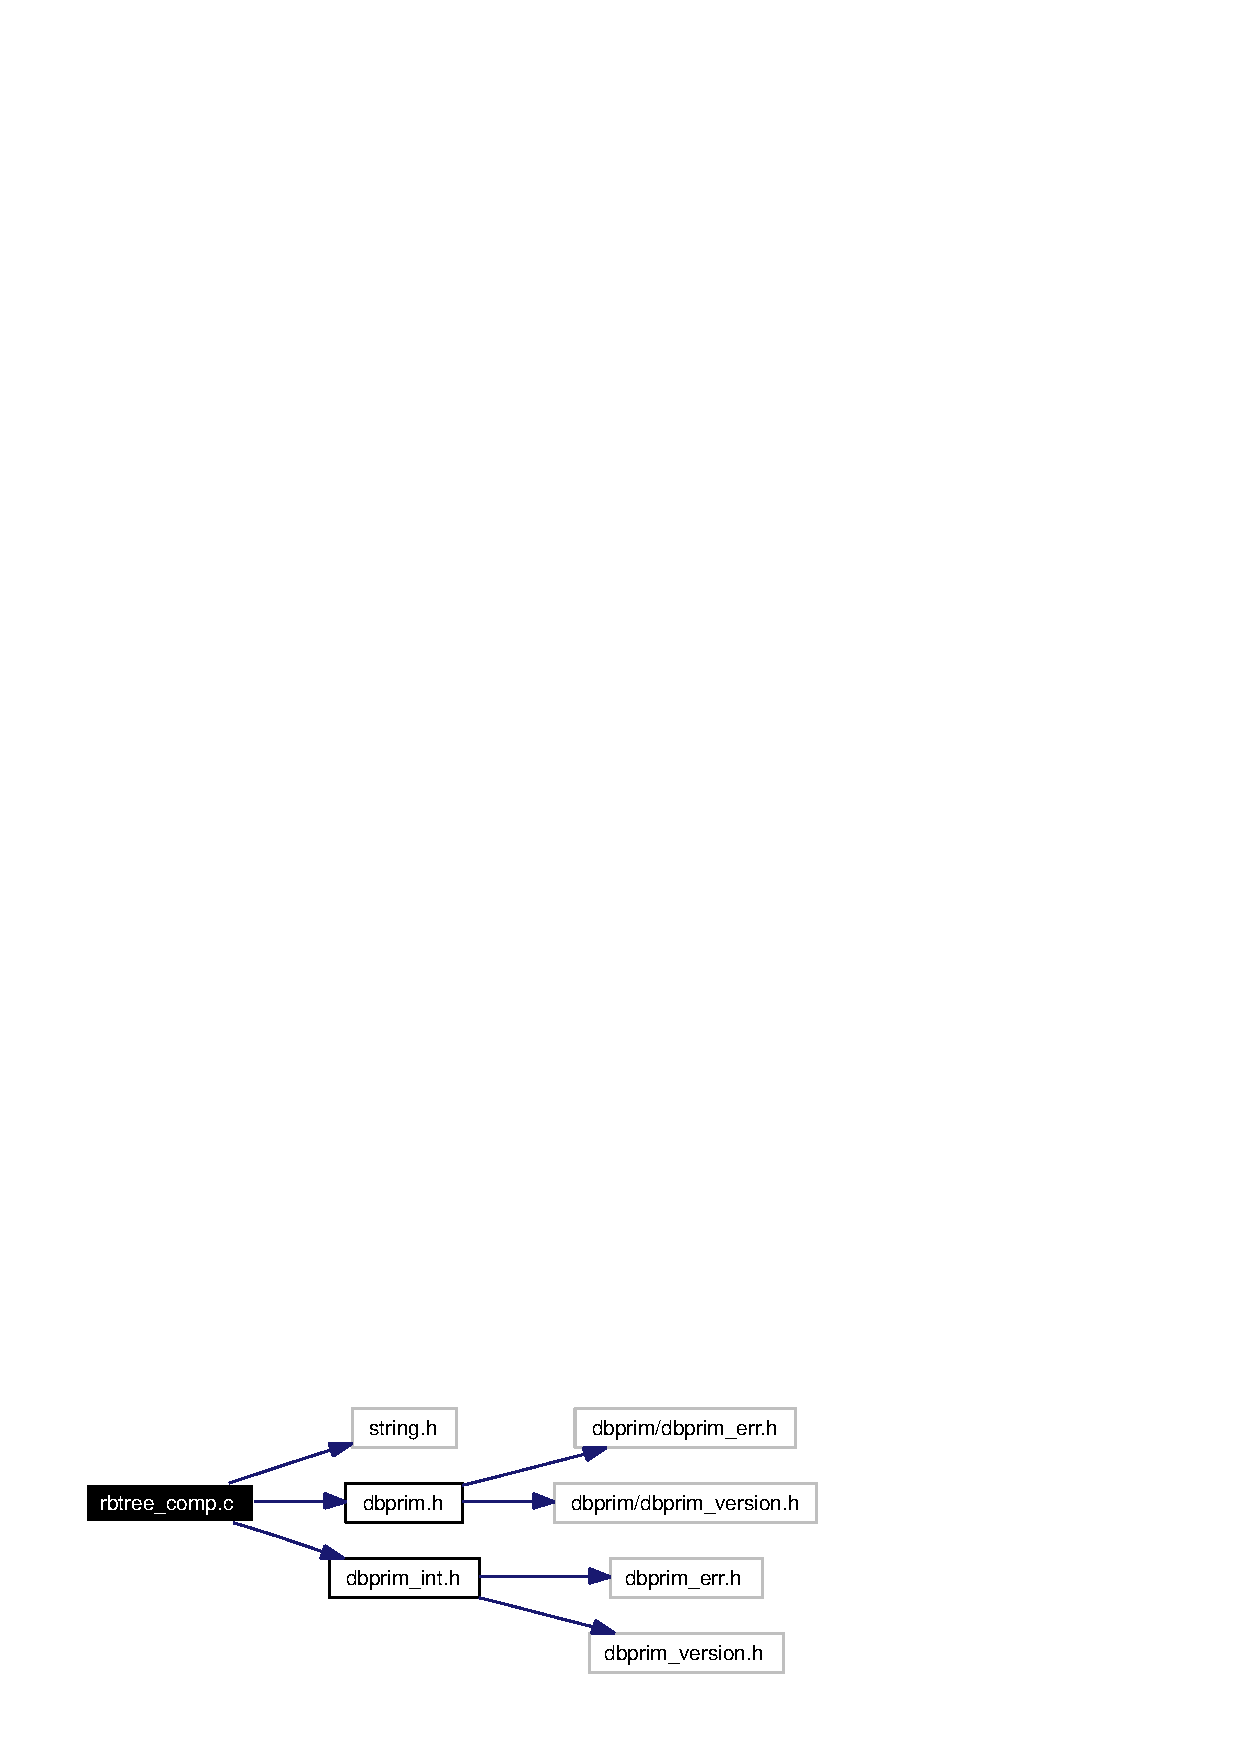
\includegraphics[width=198pt]{rbtree__comp_8c__incl}
\end{center}
\end{figure}
\subsection*{Functions}
\begin{CompactItemize}
\item 
long \hyperlink{group__dbprim__rbtree_ga5}{rbtree\_\-comp} (\hyperlink{struct__rb__tree__s}{rb\_\-tree\_\-t} $\ast$tree, \hyperlink{struct__db__key__s}{db\_\-key\_\-t} $\ast$key1, \hyperlink{struct__db__key__s}{db\_\-key\_\-t} $\ast$key2)
\begin{CompactList}\small\item\em Red-black tree comparison function. \item\end{CompactList}\end{CompactItemize}
